% %This is a very basic essay template based on array class.
\documentclass[12pt,a4paper]{article}
\usepackage{ucs}
\usepackage[T2A]{fontenc} 
\usepackage[utf8]{inputenc}
\usepackage[english,bulgarian]{babel} \usepackage[margin=1in]{geometry}
% \usepackage[bindingoffset=2cm,centering,includeheadfoot,margin=1in]{geometry}
\usepackage{graphicx}
\usepackage[unicode]{hyperref}

\addto\captionsbulgarian{%
  \renewcommand{\contentsname}%
    {Содржина}%
  \renewcommand{\tablename}%
    {Табела}%
  \renewcommand{\figurename}%
    {Слика}%
  \renewcommand{\bibname}%
    {Референци}%
  \renewcommand{\refname}%
    {Референци}%
  \renewcommand{\listfigurename}%
    {Листа на слики}%
  \renewcommand{\listtablename}%
    {Листа на табели}%
}

\title{Локацијата на корисникот во мобилните апликации\\Цената на приватноста}
\author{М-р Томче Делев}
\date{}

\begin{document}
\maketitle

Мобилните телефони се уреди кои се многу лични. Тие се наменети да ги носиме
секаде каде што одиме. Нивната врска со корисниците е многу силна. Тие се првото
нешто кое го гледаме кога се будиме, ги користиме кога ни е досадно или кога
патуваме, а понекогаш се наш основен извор на информации.

Денес стандардните мобилни телефони се повеќе се заменуваат со т.н. паметни
телефони. Овие уреди се карактеризираат со брзината на процесорот во рамките на
GHz, голема работна меморија и огромен капацитет на постојана меморија. Во нив
се вградени сензори како акселерометар, жироскоп или сензор за
осветленсот, а речиси во секој паметен телефон е вграден и сензор за сателитско
лоцирање со помош на глобалниот систем за позиционирање (GPS). Со други зборови денешниот паметен телефон може да
реагира на секое негово придвижување, менување на околината во која се користи
или пак да ја дознае вашата локација со прецизност од неколку метри. 

\begin{figure}[htb] \centering
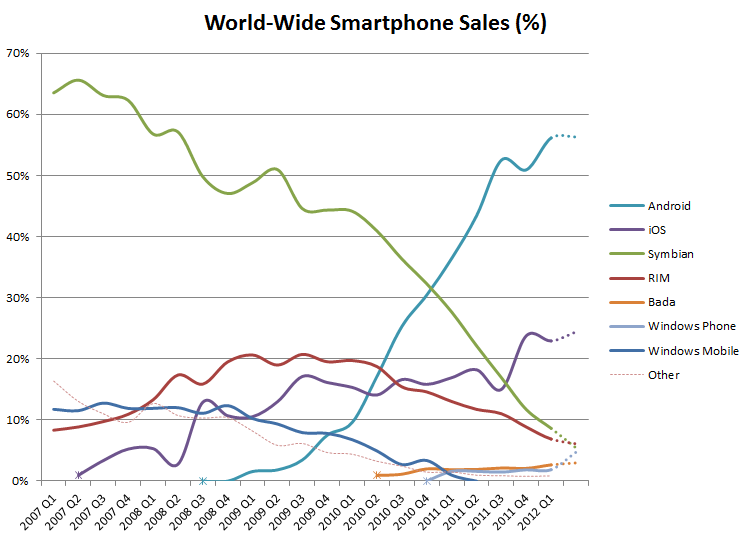
\includegraphics[scale=0.4]{images/World_Wide_Smartphone_Sales_Share}
\caption{Поделба на пазарот на продажба на паметни мобилни телефони по
платформи.}
\label{fig:market_share}
\end{figure}
Во големиот раст на пазарот на паметни мобилни телефони
(слика \ref{fig:market_share}) секако влијае и развојот на современите
платформи како iPhone OS, Android и Windows Phone. Овие платформи се составени од оперативен систем, сопствен пакет
за развој и задолжително маркет или пазар на апликации за нивната
платформа. Едноставниот модел за развој и објавување на апликации во кој со
неколку функциски повици ви се достапни сите напредни можности на паметниот
телефон, а со неколку кликови нивно објавување, предизвика интересно поместување
на мобилните телефони од едноставни уреди за комуникација во т.н. телефони за
апликации.

Од огромниот број на мобилни апликации се издвојуваат апликации кои го користат
контекстот на корисникот со цел да му понудат подобро и персонализирано
корисничко искуство. Контекстот на корисникот го сочинуваат информации како
локацијата, времето, опкружувањето и сите останати елементи во неговата
околина. Од различните видови контекст најзначјани се локацијата (каде?), идентитетот
(кој?), времето (кога?) и активноста (што?). Покрај тоа што овие информации за
контекстот одговараат на некои од најинтимните прашања за корисникот тие се и
извор на многу останати информации. На пример, ако е познат
идентитетот на корисникот, може да се дојде до неговите телефонски броеви,
адреса, е-адреса, место на раѓање, листа на пријатели и многу други приватни
информации. Ако пак е позната неговата локација, можеме да одредиме што друго се
наоѓа околу него, кои луѓе и предмети се наоѓаат во близина или кои настани се
случуваат во опкружувањето.

Можноста да се дознае или одреди локацијата на корисникот овозможува мобилните
апликации да ги прилагодат своите функционалности и сервиси на соодветната
локација и контекст. За компаниите кои нудат вакви сервиси, секоја информација
за корисникот има огромна вредност. Информацијата за локацијата се употребува за
подобро профилирање на корисникот, односно со дознавање на местото на неговото
живеење, неговото движење, неговото работно место и слично. Маркетиншката
вредноста на ваквите информации е непроценлива. Овие информации овозможуваат да
му се понудат на корисникот производи и услуги кои се во неговото опкружување и
се соодветни на неговиот стил на живот.

Еден пример на ваква мобилна апликација e SportyPal \cite{sportypal} која
интензивно споделува приватни информации за локацијата на корисникот, а притоа спаѓа во категоријата апликации добри за здравјето. Оваа апликација собира
податоци за локацијата на корисникот од неговиот мобилен телефон, кој тој го
поседува во моментот кога извршува некоја спортска или рекреативна активност со
движење на отворен простор. Со помош на овие податоци апликацијата му прикажува
поминато растојание, моментна брзина, потрошени калории итн. Но во исто време
оваа апликација го прашува корисникот дали сака да ги сподели овие информации со
нивниот сервис кој за возврат ќе понуди и дополнителни анализи и прикази. Овие
податоци може да бидат приватни или да бидат објавени јавно. Доколку вие
сте редовен корисник на апликацијата и често ја користите за возење велосипед и
притоа постојано минувате во близината на некаков бизнис за кој вашиот профил е
одличен клиент, вие станувате мета на производот на овој бизнис. Најголем дел од
овие сервиси и апликации се бесплатни. Но за апликациите кои ќе успеат да
формираат критична маса на корисници, а со тоа и доволна количина на податоци со
квалитетни информации за своите корисници, ова претставува единствен бизнис
модел за заработка и повраток на инвестицијата.

Но која е вистинската цена која ја плаќаат корисниците? Ова прашање има различни
одговори од различни аспекти. Од аспект на маркетингот постои едно интересно
гледиште на таргетираното маркетирање. Се наоѓате во пустина и се обидувате да
стигнете до првото населено место, а притоа сте очајно жеден. Дали ако во овој
случај на каков било начин ви се проследи реклама за вода на оддалеченост 1км
од вашата локација, тоа за вас ќе биде реклама или информација со огромна
вредност. Не само од аспект на компаниите кои ги продаваат личните и приватни
информации за корисниците, некогаш и самите корисници ги чувстуваат придобивките
од сервисите кои вистински ги употребуваат овие податоци. Ова е новата димензија
на маркетингот во која рекламата станува вредна информација, во која вие сте
продуктот, а бизнисот купувач.

Според Wall Street Journal\cite{appleGoogle}, Google и Apple собираат информации
за локацијата како дел од нивната трка да изградат огромни бази на податоци со
кои ќе ги лоцираат нивните корисници преку нивните мобилни телефони. Овие бази
на податоци ќе им помогнат во трката за пазарот на локациски базираните сервиси
вреден \$2.9 милијарди долари, а кој се очекува да порасне на \$8.3 милијарди до
2014. Големите компании како Google и Apple во своите полиси за приватност
\cite{applePrivacy,googlePrivacy} ги дефинираат начините на кои ги собираат
употребуваат вашите податоци за локацијата. Понекогаш овие текстови знаат да
предизвикаат загриженост на корисниците \cite{latimes}, посебно кога ќе
прочитаат извадоци како „Apple ги собира точните локации на корисниците на iPhone и iPad“.
Ваквите случаи вообичаено завршуваат со дообјаснување и доплнување на овие
полиси, со тоа дека податоците се собираат само со дозвола на корисниците и дека
тие се употребуваат анонимизирани и со цел да ги подобрат сервисите, содржината
и маркетингот. Целосната анонимизираност на податоците е посебна дилема со оглед
на успешните обиди \cite{narayanan2008robust} да се извлечат податоци за
идентитетот на корисниците единствено со помош на огормното количество податоци
кои ги поседуваат ваквите сервиси.

„Приватноста повеќе не постои. Помирете се со тоа.“ \cite{dead} оваа изрека уште
пред почетокот на овој век од страна на директорот на Sun Microsystems, само
потврдува дека со постоењето на огромни бази на податоци во секој сегмент од
нашиот живот, како и се поголемиот дигитален отпечаток кој го оставаме на
интернет, приватноста веќе го губи своето значење. Во денешно време сме
приморани да се адаптираме на една нова приватност во виртуелните општества на
социјалните мрежи и интернет.

Но дали толку лесно може да го проголтаме губењето или трансформирањето на
нашата приватност. Педесет и осум проценти од потрошувачите кои поседуваат
паметен телефон користат локациски базирани апликации и покрај загриженоста
околу безбедноста и употребата на нивните лични податоци за маркетинг
\cite{locationAppsPopular}. Од друга страна, запознаени со фактите, на прашањето
„Дали мислите дека апликациите треба да ве информираат кога тие собираат и
испраќаат информации за вашиот мобилен телефон?\cite{questionary}, 67.9\%
одговараат дека секогаш треба да бидат информирани.

Правото на приватност е едно од основните човекови права и во некои држави тоа е
загарантирано со устав. Приватноста на локацијата, како посебен вид на приватна
информација се дефинира како \emph{можноста да се спречат трети лица во
дознавањето на точната локација во моментот или во минатото}
\cite{beresford2003location}.  Во научната јавност за прашањето на приватност на
локацијата се разграничуваат две групи на пристапи. Во првата група
\cite{bettini2005protecting,gruteser2003anonymous} спаѓаат пристапи кои акцентот
го ставаат на анонимноста и безбедноста на податоците кои се споделуваат, а во
втората група \cite{smailagic2002location} се пристапите кои се обидуваат на
јасен и транспарентен начин да му овозможат на корисникот контрола над
приватните податоци за локацијата. Од аспект на типот на податоците за
локацијата кои ги споделуваат, покажано е дека корисниците повеќе се загрижени
од сервисите кои го следат нивното движење, отколку од сервисите кои само ја
знаат нивната повремена локација \cite{barkhuus2003location}.

Корисниците кои се загрижени за приватноста на своите податоци сакаат можност да
ја контролираат преку соодветни механизми. Целта е да се свесни и постојано
имаат контрола над податоците од нивниот мобилен телефон во реално време.
Едно решение \cite{forbes} предлага три нивоа на контрола: зелено светло,
отворени податоци за сите, жолто светло отворени податоци само за апликациите
кои нудат препораки и црвено светло, без дозвола за употреба на податоци кои ја
откриваат локацијата. Тековната состојба се сведува единствено на довербата на
корисниците кон компаниите кои ги собираат нивните податоци, како и
информираноста на самите корисници за начинот на кои тие се употребуваат и
споделуваат. Ова сѐуште останува само едно отворено етичко прашање, без правни
регулативи.

Живееме во ера во која луѓето поседуваат повеќе компјутери и се во секојдневна
интеракција со нив. Постојано се во потрага по апликации кои ќе им го
олеснат животот, ќе им ја зголемат продуктивноста или пак ќе бидат само еден нов
вид забава. Овие апликации постојано обработуваат огромно количество податоци, а
многу од овие податоци се лични и ја нарушуваат приватноста на корисниците. Но
според сегашното искуство ова не значи дека во иднина нема да се развиваат и
употребуваат вакви апликации и сервиси. Напротив, во новата околина на
сепристуни компјутери, во која компјутерите се во нашите телевизори, фрижидери,
автомобили, велосипеди, весници, приватноста за која знаеме веќе нема да постои
и веројатно ќе зборуваме за некаков нов вид на приватност адаптирана на третата
ера на компјутерите.

\bibliographystyle{ieeetr}
\bibliography{location_privacy}

\end{document}
